% !TEX encoding = UTF-8
% !TEX TS-program = pdflatex
% !TEX root = ../tesi.tex

%**************************************************************
\chapter{Metodologie}
\label{cap:metodologie}
%**************************************************************

%\intro{Breve introduzione al capitolo}\\

%**************************************************************
\section{Strumenti e tecnologie utilizzate}
Per poter eseguire il confronto tra le prestazioni di database relazionali e NoSQL è stato necessario preparare tutta una serie di strumenti utili a far funzionare i database stessi e al monitoraggio dei dati contenuti al loro interno.

\subsection{Docker}
Per poter effettuare test consistenti, evitare problemi di installazione e compartimentalizzare l'ambiente di lavoro, si è deciso di sfruttare Docker. Questo software permette di virtualizzare l'esecuzione di altri applicativi in ambienti chiusi e controllati, facilitando determinati processi di sviluppo. L'utilizzo di Docker in questo progetto lo rende più maneggevole e lineare.\\

\noindent Per poter utilizzare Docker è necessario prima comprendere alcune parole chiave e ciò che esse rappresentano:
\begin{itemize}
    \item Dockerfile
    \item Image
    \item Container
\end{itemize}
Il dockerfile racchiude una serie di istruzioni che servono a Docker per sapere come costruire un'immagine.\\
Questa, a sua volta, è uno snapshot del software che vogliamo utilizzare, comprese tutte le sue dipendenze, fino al sistema operativo. Questa immagine viene messa all'interno di un container per poter utilizzare il suddetto software.\\
Le immagini di molti software sono disponibili online e possono essere utilizzate come template da cui partire all'interno del dockerfile.\\
Una volta creata un'immagine è possibile usarla in quanti container si desidera, e la si può mettere a disposizione di altri utenti perché possano utilizzare lo stesso ambiente su macchine diverse.\\
In questo senso Docker è di fatto molto simile ad una Virtual Machine, con la differenza (cruciale) che mentre all'interno di una VM viene fatto girare un sistema operativo ``ospite'', ed ogni macchina virtuale ne utilizza uno a sè stante, i container di docker condividono lo stesso kernel, il Docker Engine, rendendo questo sistema molto più leggero e veloce.\\
Docker ci permette quindi di creare più container che funzionano parallelamente e possono comunicare tra loro, rimanendo indipendentementi dagli altri container e dal sistema operativo in cui eseguiamo il Docker Engine.\\

\noindent Nel caso di questo progetto, Docker risulta utile innanzitutto per gestire il funzionamento dei due DB (che saranno PostgreSQL e MongoDB), che verranno quindi inseriti in appositi container.\\
Per facilitare poi i processi di comunicazione con i DB verranno utilizzati altri due container contenenti delle interfacce grafiche per la gestione dei dati (rfispettivamente pgAdmin e MongoExpress).

\begin{figure}[htbp]
\begin{center}

\includegraphics[height=6em]{immagini/tecnologies-logos/Docker-Logo.png}
\caption{Logo di Docker}
\end{center}
\end{figure}

\subsection{PostgreSQL e tecnologie annesse}
Dopo aver scelto Docker come ambiente in cui far girare i database, alcune altre scelte legate alle tecnologie coinvolte in questa ricerca sono state prese come conseguenza.\\
Sebbene infatti sia possibile ``dockerizzare'' moltissimi software, per gli scopi di questa tesi è risultato più sensato partire da immagini pre-esistenti ed affidabili, disponibili sulla piattaforma ufficiale del software (hub-docker).\\
Questo ha permesso di non investire troppo tempo nella preparazione degli strumenti e di concentrare le risorse disponibili nell'effettivo confronto tra database.\\

\noindent Per tutti questi motivi si è quindi scelto di usare PostgreSQL come database relazionale da portare a confronto con MongoDB.\\
PostreSQL è un database relazionale open source molto robusto che si presta bene per rappresentare le prestazioni di un generico database di questa categoria. Esso è inoltre presente nell'hub di docker con un'immagine ufficiale, ed è quindi facile da far funzionare all'interno di un container a differenza di altri prodotti simili.\\
Sebbene PostgreSQL non sia utilizzato massivamente all'interno dell'azienda, risulta comunque molto simile alle sue controparti non open source, MSSQL e Oracle Server, che sono invece largamente usate all'interno di Ifin e sarebbero oggetto di una potenziale migrazione qualora i risultati di questa tesi si rivelassero convincenti.\\

\noindent Vale la pena di evidenziare che a differenza delle tecnologie che ricadono sotto la sigla ``NoSQL'', quelle legate ai database relazionali sono molto più simili tra loro, poichè condividono appunto il paradigma relazionale che sta alla base di tutte le variazioni esistenti proposte da aziende diverse in contesti diversi.\\
In questo senso, usare PostgreSQL non è una scelta incoerente con i motivi che hanno dato alla luce questo progetto.\\

\noindent Oltre al container utilizzato per il database di PostgreSQL, è necessario poter utilizzare uno strumento per effettuare operazioni su di esso.\\
Come spiegato in fase di analisi dei software proprietari di Ifin, questi sfruttano diversi framework e paradigmi per poter comunicare con i database ed operare su di essi le operazioni CRUD necessarie al funzionamento del software stesso. Considerato l'obiettivo di questa ricerca non avrebbe tuttavia senso investire tempo nel setup di un software dedicato a questi scopi.\\
Esistono infatti delle interfacce che ci permettono di interagire ``manualmente'' con i database senza fare uso di codice ed altre infrastrutture nel mezzo.\\
Per quanto riguarda PostgreSQL, la scelta è ricaduta su pgAdmin 4, un'interfaccia molto popolare e ben mantenuta, disponibile come immagine nella hub di docker per essere utilizzata all'interno di un container. È quindi sufficiente mettere in comunicazione i due container, uno per PostgreSQL e uno per pgAdmin, per avere a disposizione un ambiente completo in cui effettuare test su database relazionali.

\begin{figure}[htbp]
\begin{center}

\includegraphics[height=7em]{immagini/tecnologies-logos/postgresql-logo.png}
\caption{Logo di PostgreSQL}
\end{center}
\end{figure}

\subsection{MongoDB e tecnologie annesse}
Come già anticipato, per mettere a confronto le potenzialità dei database NoSQL rispetto a quelli di tipo relazionale è stato scelto MongoDB.\\
Anche in questo caso la scelta è stata guidata da più fattori che rendono Mongo il candidato perfetto per questa ricerca.\\
Lo schema dinamico su cui esso si basa, assieme alla struttura dei dati che permette di immagazzinare, rappresentano fattori che potrebbero migliorare il modo in cui le informazioni vengono tutt'ora gestite ed archiviate da Ifin.\\
La popolarità di Mongo determina inoltre un'abbondanza di guide e documentazione a cui fare riferimento per condurre un'analisi accurata delle sue potenzialità.\\
Infine, anche per questo database esiste un'immagine, mantenuta ufficialmente dal team di Mongo, per poterlo utilizzare come container all'interno di Docker.\\

\noindent Per quanto riguarda l'interazione con il database e l'utilizzo di operazioni CRUD al suo interno, sono stati utilizzati principalmente due strumenti.\\ 
In una fase iniziale in cui la necessità principale era quella di imparare e testare la sintassi delle operazioni sul database, un'interfaccia molto semplificata in grado di effettuare solo operazioni di inserimento e cancellazione dei dati è stata sufficiente. Si è quindi ricorso all'uso di mongo-express, un'interfaccia grafica molto basilare, il cui più grande pregio è quello di essere un software dockerizzabile, eseguibile assieme al container dedicato a MongoDB e connesso ad esso seguendo le regole già apprese per connettere interfaccia e database di PostreSQL.\\
In un secondo momento, tuttavia, tale interfaccia non è più risultata sufficiente, dato il tipo di analisi che si è voluto condurre sui risultati delle query e sul loro tempo di esecuzione.
Si è quindi deciso di passare all'utilizzo di un'altra interfaccia grafica, MongoDB Compass, questa volta esterna all'ambiente di Docker, installata direttamente sulla postazione fornita da Ifin durante il tirocinio.\\
Compass è un software sviluppato direttamente dal team di Mongo e mette a disposizione sia un'interfaccia grafica di facile utilizzo, sia un terminale da cui eseguire le operazioni più a basso livello, per poter utilizzare tutte le funzionalità che MongoDB ha da offrire.

\begin{figure}[htbp]
\begin{center}

\includegraphics[height=6em]{immagini/tecnologies-logos/MongoDB-Logo.png}
\caption{Logo di MongoDB}
\end{center}
\end{figure}

\subsection{Altri strumenti}
Oltre a quelli principali visti nelle sezioni precedenti, sono stati unilizzati altri strumenti di base per la stesura di appunti ed analisi, quali fogli di calcolo e documenti di testo, assieme ad altri software (principalmente online) per la creazione dei dati di test da inserire nei database, che verrranno spiegati in maggiore dettaglio nei capitoli successivi.\\

%**************************************************************
\section{Selezione di un ambito di confronto}
L'idea generale per effettuare il confronto tra le prestazioni di database relazionali e database NoSQL è di creare un Proof of Concept in grado di gestire i dati di uno dei software di punta dell'azienda (o comunque dati molto simili ad essi per quanto riguarda mole e contenuto), e di fare questo lavoro per entrambi i tipi di database. Una volta fatto ciò, si potranno elaborare delle query che mettano a confronto le prestazioni.\\

\noindent Viste le considerazioni fatte sui due software ``fratelli'', e considerato il risultato dei dialoghi avuti con i team leader di entrambi i progetti, la scelta è ricaduta su InvoiceChannel. Il motivo principale di questa scelta è che sebbene i due software siano piuttosto simili nella loro parte di backend, legata ai database, InvoiceChannel è un software leggermente più recente e per questo meno convoluto di LegalArchive.\\
Sebbene questi siano progetti commerciali, dotati di estensiva documentazione, è bene considerare che nel tempo allocato per effetturare lo stage non sarebbe stato possibile approfondire nel dettaglio tutti gli aspetti di questi software.\\
Per lo stesso motivo, anche una volta scelto InvoiceChannel è stato necessario condurre uno studio per identificare una piccola parte del database che esso utilizza, su cui basarsi per costruire i database necessari ai test di confronto.\\


%**************************************************************
\section{Modellazione del database relazionale}
Una volta definite queste premesse, è stato effettuato uno studio approfondito della struttura del database di InvoiceChannel, ricostruendo le relazioni tra tabelle a partire da un file in formato sql fornito dal team di test.\\
Esso contiene più di ottantamila righe di codice e definisce la struttura, il contenuto e le relazioni tra le circa 150 tabelle che compongono un database utilizzato per effettuare test di vario tipo all'interno dell'azienda.\\

\noindent Risulta ovvio come InvoiceChannel sia troppo grande e complesso per poter essere rimodellato nella sua interezza in questo contesto. Anche pensare di utilizzarne soltanto una sezione risulta piuttosto complesso, poichè tutte le tabelle sono estremamente interconesse.\\
Un ulteriore livello di complessità viene posto dalle query, anch'esse molto convolute, che fanno spesso un uso massiccio di operazioni di join.\\
L'opzione migliore è quindi ricostruire effettivamente un pezzetto di database di InvoiceChannel ad-hoc, per soddisfare le necessità del progetto, sia in formato RDBMS, sia in formato NoSQL.\\

\subsection{Definizione di tabelle e relazioni}
La sezione in questione è quella relativa alle fatture, che risulta piuttosto centrale allo scopo del software. Le tabelle coinvolte nel diagramma entità-relazione sono quelle che si occupano di immagazzinare i dati relativi alle fatture elettroniche, lo stato dei processi che le coinvolgono, i documenti ad essa collegati e l'ente che l'ha generata.\\

\begin{figure}[htbp]
\begin{center}
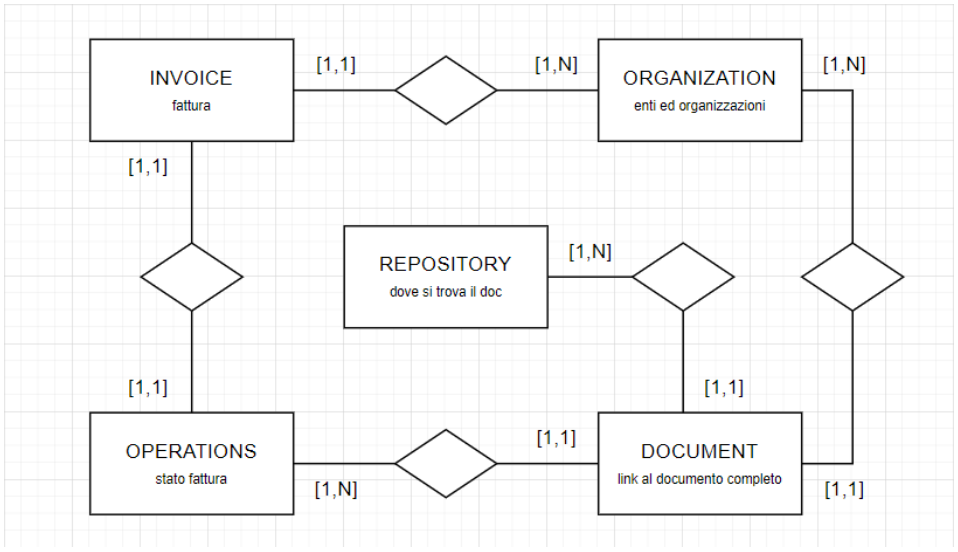
\includegraphics[height=22em]{immagini/ER-Mock-IC.png}
\caption{Diagramma ER per la sezione semplificata di InvoiceChannel}\label{img:schema-er}
\end{center}
\end{figure}

\noindent Dopo aver identificato le tabelle su cui concentrarsi per condurre lo studio e le relazioni che intercorrono fra di esse, si è passati alla definizione dei campi che compongono le suddette tabelle. Esse infatti devono essere ridimensionate per rispecchiare la sezione di database ridotto che è stata ricostruita.\\

\subsection{Script ridotti per la creazione delle tabelle}
Viene di seguito riportato il contenuto delle tabelle ristrutturate.\\

\begin{lstlisting}[language=SQL,
        deletekeywords={IDENTITY,INT},
        morekeywords={clustered},    
        framesep=10pt,
        framextopmargin=10pt, style=sql_style]
CREATE TABLE INVOICE(
    ID numeric(22, 0) NOT NULL,
    ID_OPERATION numeric(22, 0) NOT NULL,
    INVOICE_NUMBER Varchar(60) NULL,
    INVOICE_DATE Timestamp(3) NULL,
    TOTAL_AMOUNT numeric(25, 9) NULL,
    RECIPIENT_NAME varchar(255) NULL,
    DATA_INVIO Timestamp(3) NULL,
    SOURCE_FILE_NAME Varchar(255) NULL,
    TIPO_FATTURA Varchar(6) NOT NULL,
    DATA_RICEZIONE Timestamp(3) NULL,
    CAUSALE Varchar(200) NULL,
    MITTENTE Varchar(200) NULL,
    ID_ORGANIZATION numeric(22, 0) NULL,
    IS_B2B numeric(1, 0) NULL,
    TIPO_DOCUMENTO char(4) NULL,
    RIEPILOGO_IVA Text NULL,
 CONSTRAINT PK_INVOICE PRIMARY KEY ( ID )
);
\end{lstlisting}
\noindent La tabella Invoice rappresenta la fattura, con tutti i dati e i codici che essa contiene. Nella sua versione ridotta sono stati eliminati molti campi che facevano riferimento a tabelle non più collegate o dati specifici appartenenti all'ambito della fatturazione elettronica non ritenuti necessari agli scopi di questa tesi.\\

\begin{lstlisting}[language=SQL,
        deletekeywords={IDENTITY,INT},
        morekeywords={clustered},    
        framesep=10pt,
        framextopmargin=10pt, style=sql_style]
CREATE TABLE DOCUMENT(
    ID numeric(22, 0) NOT NULL,
    ID_OPERATION numeric(22, 0) NOT NULL,
    CREATION_DATE Timestamp(3) NOT NULL,
    COD_DOCUMENT Varchar(255) NOT NULL,
    PATH_FILE varchar(1024) NULL,
    ID_REPOSITORY numeric(5, 0) NULL,
    DOCUMENT_SIZE numeric(22, 0) NULL,
    ID_ORGANIZATION numeric(22, 0) NULL,
 CONSTRAINT PK_DOCUMENT PRIMARY KEY ( ID )
);
\end{lstlisting}
\noindent La tabella Document contiene una serie di dati relativi al contenuto di un documento. Ogni elemento della tabella Invoice fa riferimento infatti ad uno o più documenti, tra cui la fatura vera e propria e potenzialmente altri allegati\\

\begin{lstlisting}[language=SQL,
        deletekeywords={IDENTITY,INT},
        morekeywords={clustered},    
        framesep=10pt,
        framextopmargin=10pt, style=sql_style]
CREATE TABLE OPERATIONS(
    ID numeric(22, 0) NOT NULL,
    CREATION_DATE Timestamp(3) NOT NULL,
    MESSAGE Text NULL,
 CONSTRAINT PK_OPERATIONS PRIMARY KEY ( ID )
);
\end{lstlisting}
\noindent La tabella Operations rappresenta lo stato di processo in cui si trova fattura all'interno del sistema. Man mano che il software processa la fattura, il suo stato viene aggiornato all'interno di questa tabella.\\

\begin{lstlisting}[language=SQL,
        deletekeywords={IDENTITY,INT},
        morekeywords={clustered},    
        framesep=10pt,
        framextopmargin=10pt, style=sql_style]
CREATE TABLE ORGANIZATION(
    ID numeric(22, 0) NOT NULL,
    NAME Varchar(255) NOT NULL,
    ALIAS varchar(100) NULL,
    PARTITA_IVA Varchar(255) NULL,
    COD_ORGANIZATION_TYPE Varchar(10) NULL,
    TIPO_SOCIETA Varchar(10) NULL,
    CREATION_DATE Timestamp(3) NULL,
 CONSTRAINT PK_ORGANIZATION PRIMARY KEY ( ID )
);
\end{lstlisting}
\noindent La tabella Organization contiene informazioni riguardanti gli enti e le aziende che fanno uso del software, per poter tracciare la provenienza di una fattura e compiere moltissime altre operazioni all'interno dell'applicativo.\\

\begin{lstlisting}[language=SQL,
        deletekeywords={IDENTITY,INT},
        morekeywords={clustered},    
        framesep=10pt,
        framextopmargin=10pt, style=sql_style]
CREATE TABLE REPOSITORY(
    ID numeric(5, 0) NOT NULL,
    DEFINITION Varchar(255) NULL,
    COD_REPOSITORY_TYPE varchar(10) NULL,
 CONSTRAINT PK_REPOSITORY PRIMARY KEY ( ID )
);
\end{lstlisting}
\noindent La tabella Repository contiene informazioni riguardanti la localizzazione degli archivi che contengono i documenti. \\


%**************************************************************
\section{Modellazione del database in MongoDB}
In seguito alla costruzione del database relazionale che semplifica InvoiceChannel, si può iniziare a costruirne la controparte NoSQL seguendo il modello documentale per implementarla con MongoDB.\\

\subsection{Relazioni tra tabelle}
Sebbene sia un modello documentale, Mongo mantiene comunque la capacità di mettere in relazione documenti provenienti da collezioni diverse. Bisogna tuttavia farlo nel modo corretto perché questo porti dei vantaggi.\\

\noindent Le possibili relazioni esistenti sono tre:
\begin{itemize}
    \item One to One
    \item One to Many
    \item Many to Many
\end{itemize}
Esiste inoltre un altro concetto proposto da mongo per rappresentare moli di dati enormi: si tratta dello ``zillion'', per indicare un ``many'' ancora più grande. Le vediamo con ordine.

\subsubsection{One to One}
Sono le relazioni che intercorrono tra campi della stessa tabella, ma vengono usate anche per connettere tabelle diverse, per separare i dati secondo una determinata logica.\\
In mongo è possibile mantenere separati documenti che sono in relazione one to one, usando quindi degli identificatori, oppure è possibile inserire i documenti uno nell'altro (embedding).\\
Riassumendo:
\begin{itemize}
    \item Quando possibile è meglio embeddare, per non introdurre complessità inutile.
\end{itemize}

\subsubsection{One to Many}
Sono relazioni in cui un'entità fa riferimento a molteplici altre entità, mentre queste altre possono riferirne soltanto una.\\
Anche in questo caso ci sono due possibili approcci, o si fa embedding, o si mantengono le relazioni tramite indici.\\
Nel primo caso si può inserire il documento singolo in ogni elemento del gruppo di documenti riferiti, o in alternativa si può inserire nel singolo documento tutto il gruppo con cui era relazionato. Solitamente si fa embedding nell'entità che subisce più query.\\
Se si decide invece di gestire la relazione con un indice, si può inserire una reference a tale indice, nel lato ``one'' o nel lato ``many''. Solitamente si sceglie il lato ``many''.\\
Riassumendo:
\begin{itemize}
    \item Quando possibile è meglio preferire l'operazione di embedding, per favorire la semplicità, soprattutto se si può fare sulla collection maggiormente colpita da query.
    \item Va bene usare reference quando si mettono in relazione documenti che non hanno lo stesso grado di query associate.
\end{itemize}

\subsubsection{Many to Many}
Le relazioni ``molti a molti'' sono solitamente più complesse, ma possono/devono essere semplificate nel modello relazionale introducendo una tabella di congiunzione in modo da spezzare la relazione in due relazioni ``molti a uno'';
Nel modello documentale questo non è strettamente necessario, ma è sempre giusto chiedersi se la relazione sia fondamentale così com'è o se si può semplificare.
Riassumendo:
\begin{itemize}
    \item Preferire embedding nel lato che subisce più query.
    \item Preferire embedding per informazioni che sono primariamente statiche e che possono funzionare bene anche in caso di duplicazione;
    \item Preferire invece l'uso di reference per evitare di dover avere a che fare con la duplicazione, quando questo è un effetto indesiderato.
\end{itemize}

\subsubsection{Zillions}
Con questo termine si vuole semplicemente identificare un subset delle relazioni ``one to many'', in cui many è esponenzialmente grande. Serve un occhio di riguardo per evitare operazioni che recuperano tutti gli elementi coinvolti nella relazione, poiché questo andrebbe ovviamente a creare dei grossi rallentamenti.
Per questo motivo, in caso di relazioni fatte così non è possibile pensare a soluzioni embedded, e si può solo mantenere la relazione inserendo la reference nel lato ``zillions''.

\subsection{Pattern}
Un po come i design pattern nella programmazione ad oggetti, i pattern di modellazione dei dati sono utili per rendere questi modelli più comprensibili, basandosi su principi provati, e andando quindi a rimuovere un po' di quella parte ``artistica'' che caratterizzerebbe un lavoro meno rigoroso.\\
Per quanto riguarda questo progetto, andremo inizialmente a verificare quali sono i pattern consolidati e utili per lavorare con Mongo, e successivamente determineremo se sarà consono applicarne qualcuno. Non avrebbe senso infatti applicarli a prescindere, se il progetto si rivelasse essere già abbastanza semplice così com'è.\\

\noindent Prima di tutto, è necessario quindi specificare che l'utilizzo di pattern può causare l'introduzione di duplication, staleness e integrity issues nei dati interni al modello.\\
Questi possono essere un deterrente, specialmente nel caso di progetti semplici, ma se affrontati nel modo giusto rendono l'utilizzo dei pattern una scelta proficua.\\

\subsubsection{Primo Problema: Duplication}
Può essere il risultato dell'inserimento di documenti all'interno di altri documenti, per velocizzare le query. Spesso è una cosa negativa, se fatta senza badare alle conseguenze, ma non sempre è impossibile da gestire, anzi.\\

\noindent Ci sono casi in cui la duplicazione può essere desiderabile. Per esempio se embeddiamo l'indirizzo di spedizione nell'ordine del prodotto, questo sarà una copia dell'indirizzo dell'utente. Tuttavia l'informazione è statica e anche se l'utente cambiasse indirizzo in futuro questo non influenzerebbe gli ordini passati già ricevuti.\\
Questo porta ad una soluzione migliore rispetto al dover referenziare l'indirizzo, cosa che diventerebbe lenta e non necessaria per lo scopo dell'applicativo.\\

\noindent Altro caso è quello della duplicazione di informazioni che hanno un peso, ma questo è talmente piccolo che non provoca problemi. Per esempio embeddare gli attori all'interno dei film in cui recitano è una soluzione accettabile, poiché anche in questo caso si tratta di informazioni statiche che non dovranno essere cambiate, e poco importa se lo stesso attore dovrà essere reinserito in molteplici film. Rimane una soluzione migliore rispetto al dover gestire una relazione ``many to many'' tra attori e film in cui compaiono.\\

\noindent Ultimo caso, molto più importante, è quello in cui la duplicazione c'è ed è fastidiosa.\\
Questo è spesso il caso di dati che devono essere aggiornati nel tempo. Avere più copie di questi dati porta ad un overhead di lavoro per mantenerli coerenti. In questi casi è necessario valutare tale overhead a confronto con una soluzione che non usa il pattern in questione (che sta provocando la necessità di duplicazione), per capire quale direzione prendere.\\

\subsubsection{Secondo Problema: Staleness}
Con questo termine si intende ``l'andare a male'' dei dati, che diventano obsoleti se aggiornati troppo raramente. Fornire dei dati ``stantii'' non è certo una cosa desiderabile.\\
Si tratta di un problema che affligge i sistemi moderni a causa della grande velocità con cui i dati vengono recuperati e aggiornati. A causa di ciò non si può avere la certezza di avere l'ultimo dato aggiornato.\\
La domanda da porsi quindi è: ``quanta staleness è accettabile?''. Ovviamente dipende dal tipo di dato.\\
La soluzione è usare ``batch updates'' in modo da avere la sicurezza di fare update in un tempo fissato, e per avere la possibilità di visionare gli update tramite uno stream.\\

\subsubsection{Terzo Problema: Referential Integrity}
Solitamente si hanno problemi con questo aspetto quando si eliminano parti di documenti o tabelle, senza eliminare le loro references. Non c'è quindi la classica opzione di ``on cascade - delete'' che diamo per scontata nei database relazionali. Mongo non supporta questa funzione quindi è necessario che sia l'applicazione ad occuparsene attivamente.\\\\

\noindent Riassumendo quindi quanto visto, per ogni dato che intendiamo maneggiare dobbiamo chiederci quanto segue:
\begin{itemize}
    \item È necessario/utile duplicare quest'informazione?
    \begin{itemize}
        \item Risolvere usando batch updates.
    \end{itemize}
    \item Qual'è il livello accettabile di staleness?
    \begin{itemize}
        \item Risolvere con update basati sullo stream di aggiornamenti.
    \end{itemize}
    \item Quali parti del dato necessitano maggiormente di referential integrity?
    \begin{itemize}
        \item Risolvere o prevenire implementando transazioni o stream degli aggiornamenti.
    \end{itemize}
\end{itemize}

\noindent Andiamo ora a vedere nello specifico quali sono i Pattern che si possono applicare ad uno schema documentale, e quali sono i vantaggi che possono apportare.

\subsubsection{Attribute Pattern}
In alcuni casi, nel costruire un documento, può sorgere la necessità di creare molti campi simili ma non identici (e quindi non appartenenti ad uno stesso array, per esempio). Se poi si volesse poter cercare informazioni all'interno di questi campi in modo simultaneo, questo diventa complesso.\\
Per risolvere questo problema si usa il pattern degli Attributi. L'idea è di raggruppare in qualche modo questi campi che di fatto sono simili e contengono informazioni che ha senso mantenere raggruppate.\\

\begin{figure}[htbp]
\begin{center}
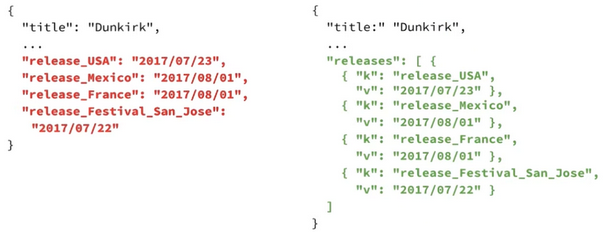
\includegraphics[height=15em]{immagini/attribute-pattern.png}
\caption{Esempio di utilizzo dell'attribute pattern}
\end{center}
\end{figure}

\noindent In questo modo si possono inserire indici ed effettuare ricerche su releases.v (per esempio).\\
I casi d'uso più comuni sono il raggruppamento di caratteristiche di un prodotto, o di un set di campi che hanno lo stesso tipo (come visto sopra per le date).

\subsubsection{Extended Reference Pattern}
Questo pattern è tra quelli che generano duplicazione nei dati, e va quindi usato con cura.
L'idea è di migliorare le operazioni che coinvolgono relazione ``One to Many''.\\
Immaginiamo di avere una relazione di quel tipo in cui, per collegare due documenti, è presente un id nell'entita ``One'' e una reference a tale id in ogni entità nel lato ``Many''. Se le operazioni che coinvolgono questi due documenti sono molto frequenti e richiedono delle informazioni che esistono solo nel lato ``Many'', saranno necessari molti join che rallentano per forza di cose l'utilizzo del DB.\\
Per ovviare a questo problema si decide quindi di rendere la reference non soltanto un campo del documento ``Many'', ma espanderla in un sottodocumento che contenga il riferimento all'id e alcuni dei campi del documento ``One'', quelli più frequentemente utilizzati nelle query, in modo da evitare il grosso dei join.\\
Tutto questo, come dicevamo, produce duplicazione di dati. Capiamo ora come gestirla.
Prima di tutto va minimizzata:
\begin{itemize}
    \item scegliendo di duplicare quei dati che non cambiano frequentemente;
    \item duplicando solo i dati necessari ad evitare le operazioni di Join.
\end{itemize}
\noindent Quando avviene un aggiornamento dell'originale:
\begin{itemize}
    \item capire quali sono le reference estese da aggiornare a loro volta.;
    \item capire quando queste reference dovrebbero essere aggiornate.
\end{itemize}
\noindent È bene inoltre tenere a mente che a volte la duplicazione è desiderabile, rispetto all'utilizzo di una normale ``singola'' reference.

\subsubsection{Subset Pattern}
Anche questo pattern si occupa di migliorare le prestazioni del DB, questa volta concentrandosi su problemi di working set.\\
Quando l'insieme di dati su cui si deve lavorare è più grande dello spazio disponibile ad accesso veloce (per esempio in RAM), il continuo scambio di informazioni con la memoria diventa un collo di bottiglia.\\
Per ovviare a questo problema, notiamo innanzitutto come in determinati casi il working set è sì troppo grande, ma è anche utilizzato solo parzialmente. Nei campi di un documento ``film'' troviamo la lista di tutto il cast, ma raramente vorremo visualizzarlo per intero. Ci basterà una lista dei 10 o 20 attori più importanti, nella maggior parte dei casi. Stessa cosa vale per le recensioni, e altri campi di questo tipo.\\
In questi casi risulta quindi utile creare un subset di questi campi, in modo da includere solo la parte importante di queste grandi liste all'interno del working set, e lasciare il resto in memoria per accedervi solo quelle rare volte che servirà, lasciando spazio a informazioni più importanti.\\
Si tende quindi a dividere le collections in due segmenti, quello con i dati più importanti e quello con i dati che ricevono meno accessi.\\

\subsubsection{Computed Pattern}
Questo pattern si basa sulla comprensione del peso che le operazioni di lettura e scrittura hanno sul sistema che si sta utilizzando.\\
In particolare, quando vengono effettuate delle operazioni (somme o altri calcoli) in fase di lettura su un set di informazioni molto ampio, questo può rendere tale lettura estremamente lenta. L'idea è quindi di tenere traccia di tali operazioni (salvandone il risultato) per poi modificarle solo in fase di aggiunta di nuove informazioni, in modo che durante la lettura il dato sia già accessibile senza nuove operazioni necessarie.\\

\subsubsection{Bucket Pattern}
Il Bucket Pattern offre una via di mezzo tra dover contenere tutte le informazioni in un solo documento, e avere un documento per ogni informazione granulare.\\
Solitamente viene utilizzato per l'IoT, dove grosse moli di dati vengono prodotte da sensori e rilevatori. Spesso si usa la data come discriminante per creare il ``bucket'' in cui raggruppare le informazioni.\\
Ci sono anche dei downside nell'introdurre questo pattern, legati al fatto che ora i dati sono separati in gruppetti, ed effettuare operazioni su tutti i dati diventa più complesso.\\

\subsubsection{Schema Versioning Pattern}
Questo pattern entra in gioco quando (non se, ma quando) arriviamo al punto di dover fare un upgrade alla struttura (schema) dei documenti. Questo processo può essere dispendioso e complesso, soprattutto per migrare i dati già esistenti nel nuovo schema.\\
Il pattern propone di procedere come segue:
\begin{itemize}
    \item Ogni documento riceve un campo ``schema-version'' che identifica la versione dello schema su cui si basa, con cui è stato costruito;
    \item L'applicazione deve poter gestire tutte le versioni di schema presenti a DB, per poter gestire il cambiamento in-itinere senza dover bloccare tutto durante la transizione ed effettuarla in un unico momento;
    \item Si sceglie una strategia di migrazione dei dati, che sia essa aspettare l'update dei singoli documenti per altri motivi e sfruttare l'occasione per mutare anche lo schema, oppure fare dei batch update appositamente dedicati a questa modifica.
\end{itemize}
\noindent Questo pattern è particolarmente utile quindi quando non ci si può permettere di avere downtime sul sistema, che deve continuare a funzionare in modo costante.\\

\subsubsection{Tree Patterns}
Il modello documentale si presta bene per rappresentare modelli gerarchici di dati.\\
All'interno di questo tipo di rappresentazione, esistono alcuni pattern utili per migliorarne l'utilizzo. Come per gli altri pattern, anche in questo caso è importante capire quali siano le necessità del sistema che stiamo modellando, in modo da fare delle scelte accorte.\\
I pattern disponibili sono:
\begin{itemize}
    \item Parent References
    \item Child References
    \item Array of Ancestors
    \item Materialized Path
\end{itemize}
\noindent Ognuno ha vantaggi e svantaggi.\\
Nel caso di Parent References, si inserisce un campo ``genitore'' in ogni nodo, che indica appunto da quale nodo discende.\\
Nel caso di Child References è invece presente un array contenente tutti i ``figli immediati'', i nodi che sottostanno a quello corrente.\\
Array of Ancestors consiste in un campo (un array appunto) che contiene il padre del nodo corrente, il padre del padre, e via dicendo fino alla radice della struttura.\\
Materialized Path è leggermente diversa dagli altri come soluzione, ma consiste nel salvare come stringa un campo contenente gli antenati del nodo corrente separati con un ``value separator'', quindi per esempio il punto. In questo modo si facilitano le operazioni, che possono sfruttare quel campo in una regular expression.\\
Ovviamente si possono applicare più pattern contemporaneamente, in base alle operazioni da svolgere, perchè ogni pattern funziona bene in determinati casi, ma può avere difficoltà in altri.\\
%In tabella sono evidenziati in verde i casi in cui l'utilizzo di un pattern risulta conveniente, rispetto ai casi in cui non sarebbe utile evidenziati in rosso.\\

\begin{comment}
\begin{center}

        \renewcommand{\arraystretch}{1.5}
    
        \centering
        \begin{longtable}{| L{3cm} | C{2.5cm} | C{2.5cm} | C{2.5cm} | C{2.5cm} |}
            
            \hline
            
            %\rowcolor{mongogreen}
            & \textbf{Parent References} & \textbf{Child References} & \textbf{Array of Ancestors} & \textbf{Materialized Path} \\
            
            \hline

            \begin{small}find ancestors of node\end{small} & \cellcolor{errorpink-light} & \cellcolor{errorpink-light} & \cellcolor{mongogreen-light} & \cellcolor{mongogreen-light} \\
            
            \hline
            
            \begin{small}find who reports to node\end{small} & \cellcolor{mongogreen-light} & \cellcolor{errorpink-light} & \cellcolor{mongogreen-light} & \cellcolor{errorpink-light} \\
            
            \hline

            \begin{small}find all nodes under node\end{small} & \cellcolor{errorpink-light} & \cellcolor{mongogreen-light} & \cellcolor{mongogreen-light} & \cellcolor{errorpink-light} \\

            \hline

            \begin{small}change data from one node to another\end{small} & \cellcolor{mongogreen-light} & \cellcolor{errorpink-light} & \cellcolor{errorpink-light} & \cellcolor{errorpink-light} \\

            \hline
        
            
            \caption{Vantaggi e svantaggi dei tree pattern in base all'operazione coinvolta}
        \end{longtable}
        
    
\end{center}
\end{comment}

\subsubsection{Polymorphic Pattern}
È un pattern semplice che sta alla base di altri pattern visti in precedenza. Affronta il problema di accorpare oggetti simili ma diversi nella stessa collezione, tenendo traccia del tipo specifico di oggetto tramite un campo apposito.\\
Ci saranno quindi una serie di campi di base condivisi tra gli oggetti e altri campi specifici, a volte contenuti in subdocuments.\\

\subsubsection{Riepilogo}
È chiaro come in base al caso d'uso, l'utilizzo di un pattern può migliorare l'architettura che sta alla base del database.

\begin{figure}[htbp]
\begin{center}
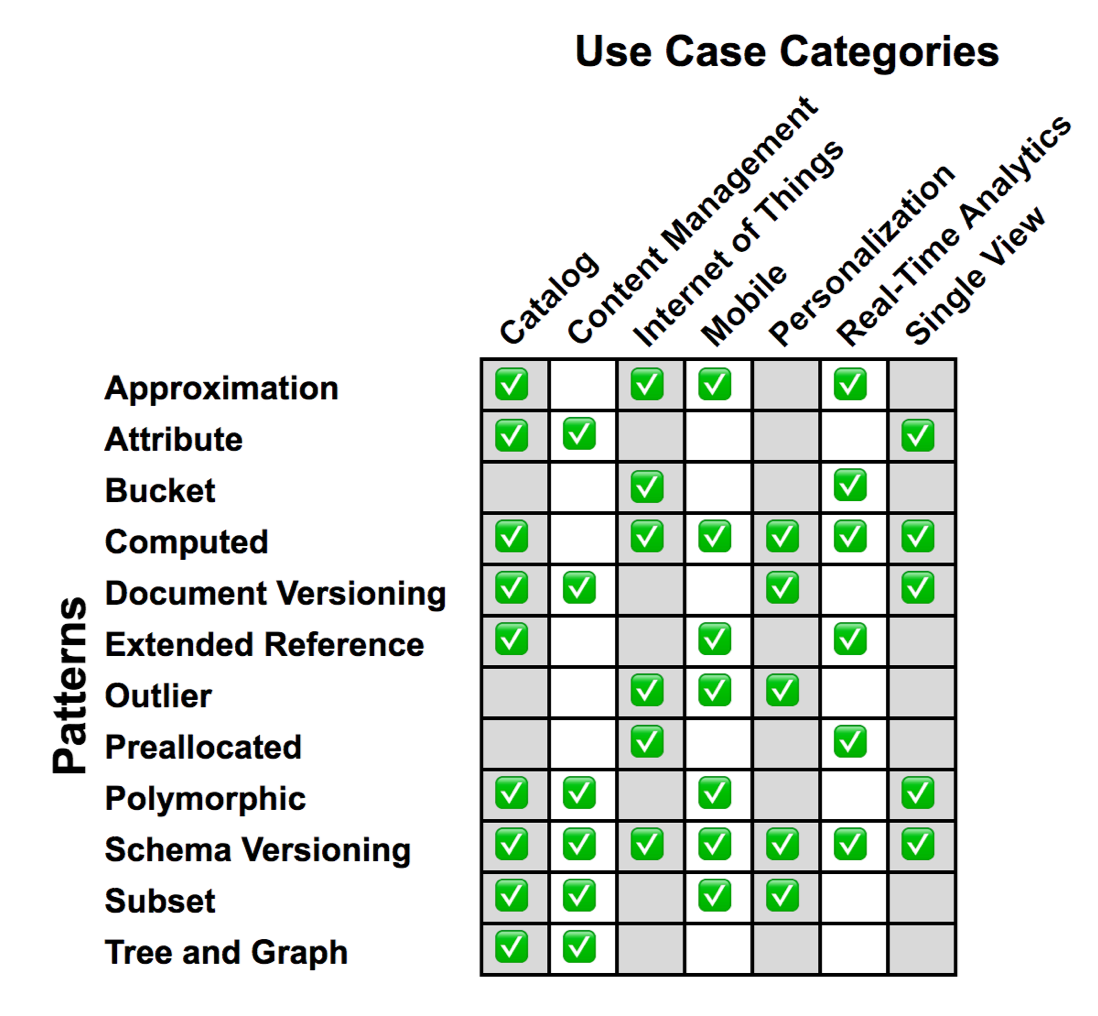
\includegraphics[height=25em]{immagini/patterns-table.png}
\caption{Applicabilità dei pattern in base al caso d'uso}
\end{center}
\end{figure}

\subsection{Migrazione del database relazionale nel modello NoSQL}
Il database relazionale costruito ed inserito all'interno di PostgreSQL è descritto dalla \autoref{img:schema-er}. Per costruire l'architettura dei documenti che risiederanno all'interno del database NoSQL, vengono riassunti i contenuti di tale figura:\\
\begin{itemize}
    \item \textbf{INVOICE} contiene dei dati relativi alla fattura inserita dall'utente;
    \item \textbf{OPERATIONS} contiene un messaggio relativo allo stato di tale fattura;
    \item \textbf{DOCUMENT} contiene il path ai vari documenti legati alla fattura, come un file di notifica del SdI, la fattura stessa, allegati, ecc;
    \item \textbf{REPOSITORY} contiene i riferimenti ai repository utilizzati per il salvataggio dei documenti;
    \item \textbf{ORGANIZATION} contiene le informazioni relative agli enti e alle aziende che usano IC. Ogni fattura o documento ``appartiene'' ad una organizzazione.
\end{itemize}

\noindent Inoltre, per quanto riguarda le relazioni che intercorrono fra le tabelle, si ha quanto segue:
\begin{itemize}
    \item INVOICE - OPERATIONS (One to One)
    \item INVOICE - ORGANIZATION (One to Many)
    \item DOCUMENT - OPERATIONS (One to Many)
    \item DOCUMENT - ORGANIZATION (One to Many)
    \item DOCUMENT - REPOSITORY (One to Many)
\end{itemize}

\noindent Dallo studio svolto sui metodi di costruzione di database documentali, si evince che l'idea generale è di accorpare, laddove possibile, più tabelle in un unico documento.\\
Questo vale per tabelle in relazione One to Many, ma soprattutto One to One.\\
Sarebbe quindi il caso di accorpare Invoice e Operations, ovvero le fatture assieme con le operazioni ad esse associate (sostanzialmente un messaggio sullo stato della fattura).\\

\noindent In base alle best practices proposte dal team di Mongo, la soluzione più coerente per costruire il database scelto per il confronto prestazionale individua tre collection separate per Invoice, Document e Organization, strutturate come segue.\\

\begin{figure}[htbp]
\begin{center}
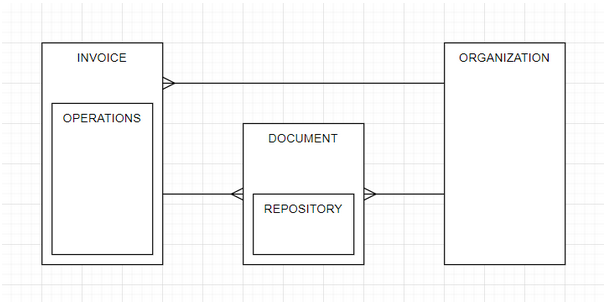
\includegraphics[height=18em]{immagini/ER-Mongo-IC.png}
\caption{Diagramma per l'architettura del database documentale}
\end{center}
\end{figure}

\noindent A seguito dello studio condotto sui pattern esistenti per la costruzione di database di questo tipo, risulta chiaro come l'aggiunta di uno di essi sarebbe una forzatura. Alcuni sarebbero indubbiamente utili qualora questo tipo di migrazione dovesse essere effettuato per componenti più corpose di InvoiceChannel, ma per quanto riguarda la parte selezionata per questa tesi, essa risulta già adeguata senza l'utilizzo di pattern.

\subsubsection{Schema del database NoSQL}
Come già detto in fase di presentazione di MongoDB, questo tipo di database documentale è spesso denominato ``schema-less''. Ciò significa che a differenza dei database relazionali, un documento all'interno di MongoDB non deve rispettare alcuno schema per strutturare i dati al proprio interno.\\
I dati sono salvati in formato JSON, sfruttando coppie di chiave valore che possono a loro volta contenere array e sotto-documenti.\\
Riportiamo quindi un esempio di documento per ognuna delle collection individuate precedentemente, per capire meglio quanto visto nel diagramma dell'architettura.\\

\noindent Esempio di documento all'interno della collection ``Invoice'':
\begin{lstlisting}[language=json,
        deletekeywords={IDENTITY,INT},
        morekeywords={clustered},    
        framesep=10pt,
        framextopmargin=10pt]
{
    "ID": "1",
    "INVOICE_NUMBER": "2",
    "INVOICE_DATE": "1986-05-16T17:36:51.514Z",
    "TOTAL_AMOUNT": "32006.83",
    "RECIPIENT_NAME": "Floor Holdings Inc",
    "DATA_INVIO": "2012-10-10T18:18:33.919Z",
    "SOURCE_FILE_NAME": "edt",
    "TIPO_FATTURA": "CA",
    "DATA_RICEZIONE": "1994-05-09T10:37:37.325Z",
    "CAUSALE": "blvd yoga bg contractor",
    "MITTENTE": "Distance Software GmbH",
    "ID_ORGANIZATION": "72",
    "IS_B2B": "false",
    "TIPO_DOCUMENTO": "TD04",
    "OPERATIONS": {
      "CREATION_DATE": "1985-03-05T20:05:37.400Z",
      "MESSAGE": "Stato fattura = Primo_Stato"
    }
}
\end{lstlisting}
\noindent Come si può notare, il documento ``Operations'' è inserito nel documento della invoice come sottodocumento. Ciò significa che alla chiave ``OPERATIONS'' corrisponde un documento innestato, al posto di un semplice valore.\\

\noindent Esempio di documento all'interno della collection ``Document''
\begin{lstlisting}[language=json,
        deletekeywords={IDENTITY,INT},
        morekeywords={clustered},    
        framesep=10pt,
        framextopmargin=10pt]
{
    "ID": "1",
    "ID_INVOICE": "462",
    "CREATION_DATE": "1970-09-18 04:42:03.000",
    "COD_DOCUMENT": "1",
    "PATH_FILE": "2",
    "DOCUMENT_SIZE": "19375",
    "ID_ORGANIZATION": "1",
    "REPOSITORY":{
        "ID": 1,
        "DEFINITION": "/home/invoicechannel/ic3/repository/repository70",
        "COD_REPOSITORY_TYPE": "HDD"
    }
}
\end{lstlisting}
\noindent Anche in questo caso esiste per ogni documento di ``Document'' un documento innestato che fa riferimento al repository di archiviazione.\\

\noindent Esempio di documento all'interno della collection ``Organization''.
\begin{lstlisting}[language=json,
        deletekeywords={IDENTITY,INT},
        morekeywords={clustered},    
        framesep=10pt,
        framextopmargin=10pt]
{
    "ID": "1",
    "NAME": "Kuphal, Rath and O'Keefe",
    "ALIAS": "1",
    "PARTITA_IVA": "4",
    "COD_ORGANIZATION_TYPE": " Azienda",
    "TIPO_SOCIETA": " Altro",
    "CREATION_DATE": "1974-01-14 08:44:54.000"
}
\end{lstlisting}
\noindent I documenti di ``Organizaion'' sono piuttosto semplici e contengono, come nella versione relazionale, le informazioni riguardanti enti e aziende che interagiscono con il sistema.\\